

\chapter{语义检查(Semantic)}
\noindent
(先写一点备注) \\
1. 强烈建议认真阅读Yx的代码和Tutorial.md。 \\
Yx是一个比Mx更加简单的语法,阅读Yx的实现对于代码的完成非常有帮助。\\
Yx的github地址:https://github.com/ZYHowell/Yx \\
2. 一些建议:多和同学、助教交流;没有头绪时多看看Yx和学长学姐的代码,有助于理解并提高效率;
切忌抄袭。\\

\section{Introduction}
在一个编译器的结构中,semantic阶段主要完成了词法分析(lexer)、语法分析(parser)、语义分析(semantic)的部分。
这一部分的评测要求是,正确地判断一段Mx代码是否存在词法、语法、语义上的错误。\\

lexer和parser的部分,我们将使用antlr4帮助我们完成;然后,我们将利用antlr4为我们生成的代码,构建AST(以下会有详解),并
进行semantic check。
接下来,我们将首先讲解对于semantic阶段工作的整体理解,再对具体的实现步骤逐步解析。

\section{Overview}
semantic部分的难点,主要在于如何构建AST。AST即abstract syntax tree,指抽象语法树。通俗地说,我们将源代转换成用树的结构来表示,
这棵树叫做AST。antlr4能够为我们完成lexer和parser,并提供接口便于我们提取其中的信息,我们希望能够自定义树的每个结点,并储存需要的
信息,所以我们将继承antlr4生成的类,然后构建一棵属于我们的AST。\\

在一切工作开始之前,我们先根据Mx语言的规定,整体了解一下我们的AST。 \\

一份Mx代码将被转换成一棵AST,这棵树从RootNode开始,随着树的层数的加深,
每层的结点所表示的单位逐渐变小。下面是基于Mx的一个AST层级的简单示意:
\begin{lstlisting}
RootNode 
- VariableDef
- ClassDefinition
    - VariableDefinition
    - FuncDefinition
- FunctionDefinition - Statements - Expressions 
\end{lstlisting}

Mx语言下,对这个结构进行一点简单的注解:\\
1. RootNode从全局作用域开始。Mx的全局作用域中只存在全局变量、类定义、全局函数三种类型。\\
2. 类定义中,只存在变量和函数。 \\
3. 一个函数包含多个statement(语句)。在AST中,一个函数中的每个statement都是这个函数节点的子节点。
statement有许多种类型,比如if语句、循环语句(for、while)等等。\\
4. expression(表达式)有许多种类型,比如基本表达式(primary)、常量表达式(constant)、赋值表达式(assignment)等等。 \\
5. 关于Mx所使用的statement和expression,Mx文档中均有明确的规定,概念模糊的同学可以先仔细阅读。 \\

如果你对以上结构感到费解,可以仔细阅读Yx库中的g4文件(Yx/src/parser/Yx.g4)辅助理解,或者继续阅读下一部分中对于如何构建AST的详细介绍,
准确地理解AST的结构将会大大提高效率。\\

\section{Practical Methods}
以下是semantic部分的具体实现过程。

\subsection{About antlr4}
antlr4是一个强大的解析器生成器。在我们的实现中,我们需要先写一个Mx.g4文件,用来描述Mx的语法,然后运行ANTLR命令,
生成MxLexer.java, MxParser.java等文件。\\

antlr4的安装、运行等等内容,请阅读《antlr4权威指南》第一部分的相应内容(pdf已下发,17页开始)。\\

antlr4的其他详细内容,请参照《antlr4权威指南》。

\subsection{Write the Grammar}
关于g4文件如何书写,《antlr4权威指南》中已经给出了详细的指导,可以结合Yx的代码理解。\\

下面结合Yx.g4,简单介绍一下g4文件各部分内容的意义(完整代码请移步Yx):\\

1. Lexer 词法分析。\\
Yx的Lexer部分如下:
\begin{lstlisting}
    Int : 'int';
    If : 'if';
    Else : 'else';
    Return : 'return';
    
    LeftParen : '(';
    RightParen : ')';
    LeftBracket : '[';
    RightBracket : ']';
    LeftBrace : '{';
    RightBrace : '}';
    
    Less : '<';
    LessEqual : '<=';
    Greater : '>';
    GreaterEqual : '>=';
    LeftShift : '<<';
    RightShift : '>>';
    
    Plus : '+';
    Minus : '-';
    
    And : '&';
    Or : '|';
    AndAnd : '&&';
    OrOr : '||';
    Caret : '^';
    Not : '!';
    Tilde : '~';
    
    Question : '?';
    Colon : ':';
    Semi : ';';
    Comma : ',';
    
    Assign : '=';
    Equal : '==';
    NotEqual : '!=';
    
    Identifier
        : [a-zA-Z] [a-zA-Z_0-9]*
        ;
    
    DecimalInteger
        : [1-9] [0-9]*
        | '0'
        ;
    
    Whitespace
        :   [ \t]+
            -> skip
        ;
    
    Newline
        :   (   '\r' '\n'?
            |   '\n'
            )
            -> skip
        ;
    
    BlockComment
        :   '/*' .*? '*/'
            -> skip
        ;
    
    LineComment
        :   '//' ~[\r\n]*
            -> skip
        ;
\end{lstlisting}
值得一提,lexer部分的书写顺序是不可以任意调换的,因为词法分析器会按照g4给出的顺序去识别每个单词。
比如,在Yx.g4的lexer部分中,仅考虑词法的定义,
`int'既可以是`Int',也可以是`Identifier',但我们只希望它被识别为`Int',所以我们将`Int'写在前面。\\

2. Parser 语法分析。\\
注意,书写这部分之前,需要充分理解semantic overview部分提到的AST结构,
以减少后续写代码时回头重新修改g4文件的次数。
Yx的Parser部分如下:
\begin{lstlisting}
program: 'int main()' suite EOF;

varDef : Int Identifier ('=' expression)? ';';

suite : '{' statement* '}';

statement
    : suite                                                 #block
    | varDef                                                #vardefStmt
    | If '(' expression ')' trueStmt=statement 
        (Else falseStmt=statement)?                         #ifStmt
    | Return expression? ';'                                #returnStmt
    | expression ';'                                        #pureExprStmt
    | ';'                                                   #emptyStmt
    ;

expression
    : primary                                               #atomExpr
    | expression op=('+' | '-') expression                  #binaryExpr
    | expression op=('==' | '!=' ) expression               #binaryExpr
    | <assoc=right> expression '=' expression               #assignExpr
    ;

primary
    : '(' expression ')'
    | Identifier 
    | literal 
    ;

literal
    : DecimalInteger
    ;
\end{lstlisting}
值得一提,代码中第一行的program表示的是一份Yx代码在全局作用域体现的结构,也是AST的根节点
中会存储的内容。Yx语言中,全局作用域内只有main函数,所以Yx.g4的program比较简单。\\

Tips: \\
1. 对于Mx,如果觉得Lexer和Parser置于同一文件中过于复杂,可以考虑分为两个文件(MxLexer.g4, MxParser.g4)来书写。
整合方法可自行查阅。\\
2. 如果你使用IDEA,可以基于你写的g4文件,输入一段Mx代码,可视化地生成解析树。效果大致如下,具体方法可自行查阅。
\begin{figure}[htbp]
    \centering
    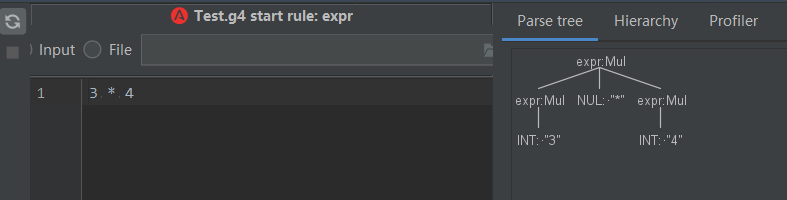
\includegraphics[width=0.7\textwidth]{image/g4.png}
    \caption{样例}
\end{figure}


\subsection{The Parse Part in compiler}
1. 生成文件解释 \\
对完成的g4文件,运行antlr4后,将生成一系列文件。下面以Yx为例对部分生成文件进行一个简单地介绍。
(建议阅读《antlr4权威指南》59页起,对生成文件的描述更加详细。) \\
 - Yx.tokens ANTLR会给我们定义的词法符号指定一个数字形式的类型,然后将他们的对应关系存储到该文件当中。\\
 - YxLexer.java 词法解析类 \\
 - YxParser.java 语法解析类 \\
 - YxListener.java, YxBaseListener.java 监听器 \\
 - YxVisitor.java, YxBaseVisor.java 访问器 \\
监听器和访问器是antlr4提供的两种遍历方法。两者的具体意义《antlr4权威指南》(49页起)有详细说明。\\

2. 调用生成代码完成lexer和parser \\
如何在我们的代码中调用antlr4生成的文件来完成lexer和paerser?Yx的main文件已经给出了示例。
下面的代码是Yx的部分代码:\\
\begin{lstlisting}
    YxLexer lexer = new YxLexer(CharStreams.fromStream(input));     // 1
    lexer.removeErrorListeners();                                   // 2
    lexer.addErrorListener(new YxErrorListener());                  // 3    
    YxParser parser = new YxParser(new CommonTokenStream(lexer));   // 4
    parser.removeErrorListeners();                                  // 5
    parser.addErrorListener(new YxErrorListener());                 // 6
    ParseTree parseTreeRoot = parser.program();                     // 7
\end{lstlisting}

3. 自定义error \\
antlr4在lexer和parser的过程中,能够发现词法、语法错误,而具体的异常类可以自定义。
这里可以参考Yx对于YxErrorListener类的处理。

\subsection{Design and Build the AST}
这部分的代码相当琐碎,且涉及到你对AST结构的理解,可以结合Yx代码仔细研究。

\subsubsection{ASTNode}
现在,我们需要建一棵AST。那么首先,我们需要为每一个节点定义一个类,来保存各自需要的信息,
从而构成一棵树。这里的树形结构和g4的语法结构本质上是一致的。\\
以下是Yx给出的ifStmtNode类的定义作为例子:
\begin{lstlisting}
    package AST;

    import Util.position;
    
    public class ifStmtNode extends StmtNode {
        ExprNode condition;
        StmtNode thenStmt, elseStmt;
    
        public ifStmtNode(ExprNode condition, StmtNode thenStmt, StmtNode elseStmt, position pos) {
            super(pos);
            this.condition = condition;
            this.thenStmt = thenStmt;
            this.elseStmt = elseStmt;
        }
    
        @Override
        public void accept(ASTVisitor visitor) {
            visitor.visit(this);
        }
    }
\end{lstlisting}


\subsubsection{ASTBuilder}
在上述的Parse Part结束后,antlr4生成的代码为我们构建了一棵parse tree(即parseTreeRoot)。
你可以认为,parse tree已经具有一个理想的树的结构,但是它保存的信息不足以满足我们的需求,
故我们仍然需要建立一个AST,读取parse tree并增添我们需要的内容。\\

antlr4生成的文件中,MxBaseVisitor提供了可以显式访问parse tree子结点的接口,所以
ASTBuilder类将继承MxBaseVisitor类,然后访问parse tree的各个节点,将
需要的信息依次读入自定义的各种ASTNode类中,构建自己的AST树。\\

关于MxBaseVisitor提供的接口如何使用,可以参考Yx代码。 \\

以下是Yx给出的一个例子:
\begin{lstlisting}
@Override public ASTNode visitVarDef(YxParser.VarDefContext ctx) {
    String name = ctx.Identifier().toString();
    ExprNode expr = null;
    if (ctx.expression() != null) expr = (ExprNode)visit(ctx.expression());

    return new varDefStmtNode(name, expr, new position(ctx));
}
\end{lstlisting}


\subsubsection{Scope}
Scope表示作用域。一般而言,由 \{ 和 \} 组成的块会引进一个新的作用域,当然,在Mx文档中关于作用域有更加详细准确的描述。\\

对于我们semantic阶段的实现来说,处理Scope的意义是,我们需要保存每个作用域内定义的变量、函数等等信息,
来确保每次在当前作用域或者更内层的作用域中调用某个变量或函数时,我们能够找到它们对应的定义,并判断是否存在语义错误
(类型错误、重名等问题)。\\

在Yx的示例代码中,关于Scope采用了一个类似树的结构来维护,根据作用域的关系建树。
具体的实现思路是:定义一个Scope类,用以储存每个作用域内需要的信息。
以全局作用域作为根节点。维护一个currentScope表示当前作用域,如果产生了一个新的作用域(比如
在IfStmtNode中,一个if-else语句会产生两个内层的作用域),则新建一个Scope类变量作为新的currentScope,完成
该内层作用域内的工作后,再将currentScope退回先前的作用域,通过成员变量parentScope记录作用域之间的关系并实现回溯。
这样,每当我们需要为一个被调用的变量寻找它的定义,我们可以通过parentScope从当前作用域不断向前回溯,直到找到
这个变量对应的定义。\\

需要强调,Mx语言中内层作用域可以遮蔽外层作用域的名字,这也是我们采用上述方法来实现Scope的一个重要原因。\\

Yx关于Scope类的定义在 Yx/src/Util/ 中,如果对以上的描述感到困惑,可以结合Yx的代码对这一部分进行理解。

\subsection{Semantic}
进行到这一步,我们已经建好了AST,接下来我们将进行语义检查。\\

\subsubsection{SymbolCollector}
首先,我们提出 type system 这一概念。在Mx语言中,允许出现的类型除了Mx文档提到的int,bool等基础类型外,还会
出现Mx代码中自定义的类。所以我们需要建立一个 type system来管理各种类型。\\

对于type system这一概念的实现,Yx的方法是,写一个Type类用来表示类型,然后维护一个globalScope类(一个继承Scope的类
,表示全局作用域)变量,
在SymbolCollector类中,将Mx的基本类型和代码中的自定义类型用Type表示,并保存在globalScope类变量中。 \\

SymbolCollector类是一个全局作用域内的收集,它存在的意义是,Mx会在全局自定义类,自定义类也会出现在各个函数和变量定义中,包括出现在其他的类定义中,作为变量类型或者函数的返回类型,所以
在遍历AST进行语义检查之前,我们需要先收集并保存所有的自定义类。当然,收集过程中也需要做一些语义检查,比如重名、出现不存在的类型等。 \\

值得一提,之所以将这部分从SemanticChecker独立出来,是因为 收集自定义类 这个步骤,需要在 遍历所有节点并进行语义检查 之前进行,
是管理type system的一个类。事实上,这部分的设计非常自由,你可以进行更多你认为合理的操作。\\

如果你对以上内容感到费解,可以阅读Yx的Tutorial.md中的讲解和Yx代码,辅助理解。

\subsubsection{SemanticChecker}
现在,AST的信息和type system,我们开始进行语义检查。 \\

我们在ExprNode(表达式节点)中加入了一些成员变量,帮助我们处理一些语义错误,比如: \\

1. 用`type'表示每个`ExprNode'的类型,用来处理类型匹配问题。\\
例如:表达式`a==b' (`a'与`b'都是int型)的类型是bool型的,
所以它的`type'应为bool型。\\

2. 用`isAssignable'表示每个`ExprNode'是否能够被赋值,用来处理右值问题。\\
例如:表达式`++a'可以作为左值,是可以被赋值的;而表达式`a++'只能作为右值,`a++ = 1'这样的表达式是非法的。\\

Mx涉及的语义错误在Mx文档中有详细的描述,这部分的代码相当琐碎,书写和debug过程中请保持耐心和细心。
具体代码可以参考Yx。





